


\documentclass{article}[12pt]
\usepackage{fullpage,graphicx, setspace, latexsym, cite,amsmath,amssymb,color,subfigure}
%\usepackage{epstopdf}
%\DeclareGraphicsExtensions{.pdf,.eps,.png,.jpg,.mps} 
\usepackage{amssymb} %maths
\usepackage{amsmath} %maths
\usepackage{amsthm}
\usepackage{mathtools}

\bibliographystyle{unsrt}
\usepackage{hyperref}
% \bibliographystyle{apj_hyperref}
\newcommand{\eprint}[1]{\href{http://arxiv.org/abs/#1}{#1}}
\newcommand{\ISBN}[1]{\href{http://cosmologist.info/ISBN/#1}{ISBN: #1}}
\newcommand{\adsurl}[1]{\href{#1}{ADS}}
\providecommand{\url}[1]{\href{#1}{#1}}



%notation
\usepackage[draft]{commands}
% \newtheorem{theorem}{Theorem}
% \newtheorem{prop}{Proposition}
% \newtheorem{corollary}{Corollary}
% \newtheorem{lemma}{Lemma}
% \newtheorem{defn}{Definition}
% \newtheorem{ex}{Example}
% \usepackage{float}

% \def \A{\cal A}
% \def\R{\mathbb{R}}
% \def\Eps{\mathcal{E}}
% \def\E{\mathbb{E}}
% \def\V{\mathbb{V}}
% \def\F{\mathcal{F}}
% \def\G{\mathcal{G}}
% \def\H{\mathcal{H}}
% \def\S{\mathcal{S}}
% \def\P{\mathbb{P}}
% \def\1{\mathbf{1}}
% \def\n{\nappa}
% \def\h{\mathbf{w}}
% \def\v{\mathbf{v}}
% \def\x{\mathbf{x}}
% \def\X{\mathcal{X}}
% \def\Y{\mathcal{Y}}
% \def\eps{\epsilon}
% \def\y{\mathbf{y}}
% \def\e{\mathbf{e}}
% \newcommand{\norm}[1]{\left|\left|#1\right|\right|}
% \DeclareMathOperator*{\argmin}{arg\,min}
% \DeclareMathOperator*{\argmax}{arg\,max}

\newcommand{\lecture}[4]{
   \pagestyle{myheadings}
   \thispagestyle{plain}
   \newpage
   % \setcounter{lecnum}{#1}
   \setcounter{page}{1}
   \setlength{\headsep}{10mm}
   \noindent
   \begin{center}
   \framebox{
      \vbox{\vspace{2mm}
    \hbox to 6.28in { {\bf ESE 680-004: Learning and Control
   \hfill Fall 2019} }
       \vspace{4mm}
       \hbox to 6.28in { {\Large \hfill Lecture #1: #2  \hfill} }
       \vspace{2mm}
       \hbox to 6.28in { {\it Lecturer: #3 \hfill Scribes: #4} }
      \vspace{2mm}}
   }
   \end{center}
   \markboth{Lecture #1: #2}{Lecture #1: #2}

   \noindent{\bf Disclaimer}: {\it These notes have not been subjected to the
   usual scrutiny reserved for formal publications. }
   \vspace*{4mm}
}

\begin{document}

\lecture{12}{Learning to Control Markov Decision Processes}{Nikolai Matni}{Klayton Wittler}

\section{Introduction}
Previously we were able to show with system level synthesis and robust control bounds \cite{AndersonEtAl19} that end-to-end guarantees of performance for a controller

\begin{equation}
    \frac{\hat{J} - J_{*}}{J_{*}} \leq C(robustness, excitability) \sqrt{\frac{(d+p)\log{\frac{1}{\delta}}}{N}}
\end{equation}

with probability of $1- \delta$ for sufficiently large N. Here $\hat{J}$ represents the learned controller on the true system, $J_{*}$ is the optimal performance, d is the number of states and p is the number of inputs, and C is a constant depending on the true system.

\begin{figure}[h!]
    \centering
    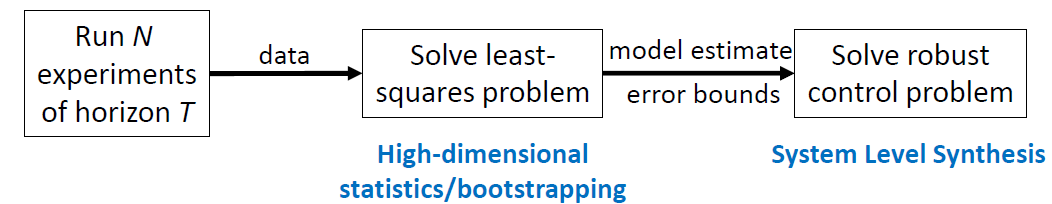
\includegraphics[scale=0.4]{images/end2end.png}
    \caption{Learning and control pipeline}
    \label{fig:end2end}
\end{figure}

However to understand how good this guarantee is we need to understand different performance metrics for learned control policies. 

\section{MDP}
\subsection{Finite MDP}
In finite MDP we consider the following equation where $T$ is the horizon length.

\begin{equation}
\begin{split}
   \min_\pi & \E [\sum_{t=0}^{T-1} c_t(x_t,u_t) + c_T(x_T) ]\\
    \st & x_{t+1} = f_t(x_t, u_t, w_t) \\
   & u_t = \pi_t(x_{0:t},u_{0:t-1})
\end{split}
\end{equation}

Here $x_t \in \R^{n_x}$ is the state, $u_t \in \R^{n_u}$ the control input, and $\w_t \in \R^{n_w}$ the the state transition noise. The control policy is $\mathbf{\pi} = \{\pi_1,...,\pi_t,..,\pi_{T-1}\}$ where a particular $\pi_t$ maps the current state and previous inputs to the current input and is possibly a random mapping.

If dynamic transition functions and cost functions are known and Markovian we can restrict the policy search to $u_t = \pi_t(x_{t})$ and solve using dynamic programming via Bellman iteration on the value function.
\begin{equation}
\begin{split}
V_T(x_T) &= \E[c_T(x_T)] \\
V_t(x_t) &= \min_{u_t} \E[c_t(x_t,u_t) +  V_{t+1}(f_t(x_t,u_t,w_t))]
\end{split}
\end{equation}


In the example of the Linear Quadratic Regulator (LQR) with time invariant dynamics and cost, $Q \succ 0$, and $R \succ 0$.

\begin{equation}
\begin{split}
   \min_\pi & \E [\sum_{t=0}^{T-1} x_t^TQx_t + u_t^TRu_t + x_T^TQ_Tx_T ] \\
   \st & x_{t+1} = Ax_t + Bu_t , x_0 = \zeta \\
   & u_t = \pi_t(x_{t})
\end{split}
\end{equation}


where $V_T(x) = x_T^TQ_Tx_T$ and assume $V_{t+1} = x_{t+1}^TP_{t+1}x_{t+1}$ to solve the recursion on

\begin{equation}
    \begin{split}
       V_t(z) &= \min_u z^TQz + u^TRu + V_{t+1}(Az+Bu) \\
       &= \min_u z^TQz + u^TRu + (Az+Bu)^TP_{t+1}(Az+Bu) \\
       &= z^T(Q+A^TP_{t+1}A-A^TP_{t+1}B(R+B^TP_{t+1}B)^{-1}B^TP_{t+1}A)z
    \end{split}
\end{equation}

with 

\begin{equation}
    \begin{split}
        u_t^* &= Kx_t \\
        K &= -(R+B^TP_{t+1}B)^{-1}B^TP_{t+1}A \\
        P_t &= Q+A^TP_{t+1}A-A^TP_{t+1}B(R+B^TP_{t+1}B)^{-1}B^TP_{t+1}A \\
        P_T &= Q_T
    \end{split}
\end{equation}


\subsection{Infinite MDP}
Moving to the infinite horizon setting with static cost and dynamics functions then different infinite horizon costs can be formulated.

The discounted cost setting:

\begin{equation}
\begin{split}
    &\E[\sum_{t=0}^{\infty} \gamma^t c(x_t,u_t)] \\
    &\gamma \in \left(0,1\right]
\end{split}
\end{equation}

If $c(x_t,u_t)$ is bounded almost surely and $\gamma < 0$ then $\E[\sum_{t=0}^{\infty} \gamma^t c(x_t,u_t)] < \infty$ which is easy to work with theoretically. The optimal cost-to-go and policy can also be obtained from the Bellman Equation
\begin{equation}
    V_*(x) = \min_u \E[c(x,u) + \gamma V_*(f(x,u,w))]
\end{equation}
which is a model-based approach using the value function and the model free approach being 
\begin{equation}
\begin{split}
    Q_*(x,u) &= \min_v \E[c(x,u) + \gamma Q_*(f(x,u,w),v)] \\
    \pi_*(x) &= \argmin_u Q_*(x,u)
\end{split}
\end{equation}
The downside being for control the bounded discounted cost does not guarantee stability.

Asymptotic average cost:
\begin{equation}
\begin{split}
    &\E[\lim_{T\rightarrow \infty} \frac{1}{T}\sum_{t=0}^{T-1} c(x_t,u_t) + c_T(x_T)] \\
    &\gamma \in \left(0,1\right]
\end{split}
\end{equation}

Care must be taken to make sure the limit converges but if the closed loop system is stable then it will converge. It is also appropriate for stability in stochastic control, but is difficult to work with theoretically. One application is in stochastic LQR below.

\begin{equation}
\begin{split}
   \min_\pi & \lim_{T \rightarrow \infty} \frac{1}{T}\E [\sum_{t=0}^{T-1} x_t^TQx_t + u_t^TRu_t + x_T^TQ_Tx_T ] \\
   \st & x_{t+1} = Ax_t + Bu_t \\
   & u_t = \pi_t(x_{t})
\end{split}
\end{equation}

which can be solved with Discrete Algebraic Riccati (DAR) recursion similar to as before. Also if $A$, $B$, and $Q^{\frac{1}{2}}$ are stabilizable and detectable then the closed loop system is stable and converges to a stationary distribution and static policy.

\section{MDP with unknown dynamics}
Now if the dynamic transition functions are unknown but the cost functions are known and time invariant, then learning can be broken into two categories episodic tasks and single-trajectory tasks. In episodic tasks data is collected over a finite horizon, updates are made, and the system is reset to begin the next episode. In single-trajectory tasks a system is evaluated under a policy during a single evolution. 

There exist a tension between identifying an unknown system and controlling it known as the exploration vs. exploitation tradeoff. Exploration requires sufficient excitation of a system to achieve an accurate model but this degrades performance and if an incorrect model is exploited then a system is left with sub-optimal performance. To quantify this tradeoff, there are two main performance metrics Probably Approximately correct (PAC) bounds and Regret bounds.

\subsection{PAC}
Tasks are performed over a horizon $H$ which may be infinite but the system can be reset after some time $H_r$. The optimal achievable cost is $V_*$ and the number of episodes for which the policy $\pi$ is not $\epsilon$-optimal ($V_{\pi} > V_{*} + \epsilon$) is $N_\epsilon$. A policy is said to be episodic ($\epsilon$,$\delta$)-PAC if after T episodes it satisfies

\begin{equation}
    \Pr[N_{\epsilon} > \poly(n_x,n_u,H.\frac{1}{\epsilon},\frac{1}{\delta})] \leq \delta \\
\end{equation}

which guarantees the chosen policy is $\epsilon$-optimal on all but a number of episodes polynomial in the parameters with probability at least $1-\delta$. The algorithm normally operates in two phases, pure exploration to approximate the system model then a exploitation where the model is used to create a control policy. Informally, PAC can be thought of the number of episodes required to have an $\epsilon$-optimal policy. 

Utilizing PAC bounds for LQR can be done for both an episodic set up as well as in the single-trajectory case. Previously in \cite{DeanEtAl17} its been shown that LQR with asymptotic average cost is episodic PAC-learnable via injecting white in time Gaussian noise to the open-loop system over at most $\poly(n_x,n_u,H_r,\frac{1}{\epsilon},\log{\frac{1}{\delta}})$ episodes followed by least-squares system identification and the robust synthesis method to guarantee

\begin{equation}
    \Pr[V_{\pi} - V_{*} \geq \epsilon] \leq \delta
\end{equation}

which can be restated in the robust synthesis framework as $\hat{J} - J_{*} \underset{\sim}{<} J_{*}O(\epsilon)$ with probability at least $1-\delta$ as long as $N \underset{\sim}{>} \frac{\sigma_{w}^2(n+p)\log{\frac{1}{\delta}}}{\lambda_{min}(\Lambda_C)\epsilon^2}$. Where as defined earlier $\hat{J}$ represents the learned controller on the true system, $J_{*}$ is the optimal performance, d is the number of states and p is the number of inputs, and 

Similarly, in a single-trajectory over an infinite horizon a policy $\pi$ can be characterized as PAC-learnable if

\begin{equation}
   \Pr[N_{\epsilon} > \poly(n_x,n_u,\frac{1}{\epsilon},\frac{1}{\delta})] \leq \delta
\end{equation}

Which guarantees the number of time-steps, $N_{\epsilon}$, where $V_{\pi}(x_t) > V_{*}(x_t) + \epsilon$ to be less than $poly(\frac{1}{\epsilon},\log{\frac{1}{\delta}})$ with probability $1- \delta$. Where $V_{\pi}(x_t)$ represents the cost-to-go from state $x_t$ achieved by a policy and $V_{*}$ is the optimal cost-to-go that can be achieved.

The limits of PAC bounds is that it is only penalized for sub-optimality above $\epsilon$ and is not guaranteed to converge to optimal since it can ceases learning after it is $\epsilon$-optimal.

\subsection{Regret}
Regret bounds evaluate the quality of an adaptive policy by comparing its running cost to a baseline. Here $b_T$ is the baseline cost at time T to be compared to the regret incurred by a policy.

\begin{equation}
    R^{\pi}(T) \coloneqq \sum_{t=0}^{T} c_t(x_T,\pi_t(x_{0:t},u_{0:t-1})) -b_T\\
\end{equation}

The two most common regret guarantees are expected regret 

\begin{equation}
    \E[R^{\pi}(T) \leq poly(n_x,n_u,T)]
\end{equation}

and high probability regret.

\begin{equation}
    \Pr[R^{\pi}(T) \geq poly(n_x,n_u,T,\frac{1}{\delta})] \leq \delta
\end{equation}

Regret bound for LQR are in the form of 

\begin{equation}
    R^{\pi}(T) \coloneqq \sum_{t=0}^{T} x_t^TQx_t + u_t^TRu_t - TV_*\\
\end{equation}

with  $V_*$ being the optimal asymptotic average cost achieved by the true optimal LQR controller. The policy from this can be shown to be $u_t = \hat{K}x_t + \eta_t$, where $\hat{K} = dlqr(\hat{A},\hat{B},Q,R)$ is the solution to LQR with estimated dynamics and has exploration in the form of $\eta_t \sim \Ncal(0,\sigma_{\eta,t}^2 I)$ which injects some noise into the control input. This achieves a regret bound of 

\begin{equation}
    R^{\pi}(T) \leq poly(n_x,n_u,\log(\frac{1}{\delta}))O(T^{\frac{1}{2}})
\end{equation}

Similarly, moving this again to the robust synthesis framework $\hat{J}_T - TJ_* \leq \Tilde{O}(T^{2/3})$ for moderate uncertainty \cite{DeanEtAl18} and $\hat{J}_T - TJ_* \leq \Tilde{O}(T^{1/2})$ for small uncertainty \cite{ManiaEtAl19}.


% Recall that least-squares estimator for a single trajectory

% \begin{equation}
%     (\hat{A},\hat{B}) \in \argmin_{A,B} \frac{1}{2}\sum_{t=0}^{T-1}\norm{x_{t+1} - Ax_t - Bu_t}_2^2
% \end{equation}

% and suppose we are given an initial uncertainty bound $\max\{\norm{\hat{A}-A},\norm{\hat{B}-B}\} \leq \epsilon_0$ so that a robustly stabilizing controller $K_0$ can be synthesized. Given the control policy $u_t = \hat{K}x_t + \eta_t$ earlier for sufficiently large $T \geq \Sigma(n_x+n_u+n_x \log{\frac{1}{\delta}(1+\sigma_u^2 \frac{\norm{B}^2}{\sigma_w^2})}$ [SimchowitzEtAl18], $ \epsilon = \max\{\norm{\hat{A}(T)-A},\norm{\hat{B}(T)-B}\} \leq \Tilde{O}(\frac{1}{\sigma_{eta}T^{1/2}})$ can be satisfied with high probability.

The limits of regret bounds is that it has no worst-case guarantee because it only tracking the integral of sub-optimal behaviour and cannot distinguish between a few severe mistakes and many small ones. However it is different from PAC in that all sub-optimal behaviour is tracked so a balance between exploration and exploitation must be made.

\subsection{Uniform-PAC}
To handle the downsides of both PAC and Regret bounds a new framework was proposed in \cite{DannLattimoreBrunskill17} to satisfy both PAC and high probability regret bounds. This is done by simultaneously for all $\epsilon > 0$ selecting an $\epsilon$-optimal policy on all episodes except for a number that scales polynomially with $\frac{1}{\epsilon}$ with high probability. The key insight into proving these bounds is to leverage time-uniform concentration bounds such as the finite-time versions of the law of iterated logarithm which gives horizon-dependent confidence levels.
%


\bibliography{ref}

 \end{document}






